\section{Discussion}

\subsection{Experiment 1 : Charging by induction}

\textbf{Part 1}

When the distance between the charged and sampling sphere was 50 cm, it was expected that the charged sphere would have little to no effect on the sampling sphere. This expectation was accurate, as the charge on the sampling sphere was uniform, as seen in Table 1. The results were, however, slightly noisy and variable; with the maximum overall residual of the average of the entire sphere being 0.68 V. In contrast, the maximum error was small, being 0.12 V. Point E, closest to the charged sphere, had a charge of 0.08 V, while point F, furthest from the charged sphere, had a charge of 0.48 V. This difference can be attributed to the sources of error discussed in the results section.\\ 
\textbf{Part 2}

The distance between the spheres was reduced to 1 cm for this part of the experiment. The charged sphere was now close enough to attract the charge of the sampling sphere. Therefore, it was expected that the electrons on the surface of the sampling sphere would be attracted to the positive charge of the other sphere, resulting in the side closest to the charged sphere (point E) to gain a negative charge distribution. Due to the charged sphere, more electrons would be situated on the side closest to the charged sphere than on the rest of the sampling sphere, causing an electric dipole. This electric dipole means that the point furthest away from the charged sphere (point F) is the most positively charged, and the point closest to the charged sphere (point E) is the most negatively charged.

The results, which can be seen in Table 2, support the expected theoretical values. The left side of the sampling sphere (point E) had an average charge of -6.28 V, and the right side (point F) had an average positive charge of +0.76 V. This non-uniform charge density is in line with the expected result. Points A, B, C and D had average voltages of +0.44, -1, +0.28 and +0.02 volts respectively. However, the negative charge on point B is understandable, because it was measured at the bottom left (closer to the charged sphere), as the stand prevented proper measurement. Due to the noisy results, the greatest maximum error and maximum absolute residual out of all the points were reasonable values of 0.44V and 0.98V, respectively. Therefore, the results match the theoretical expectations where a larger and denser negative charge is closest to the charged sphere, and a more distributed positive charge is furthest from the sphere. \\
\textbf{Part 3}

For this part of the experiment, the distance between the two spheres was kept to 1cm, but the sampling sphere was momentarily grounded whilst still close to the charged sphere. The electric dipole of the sampling sphere meant the electrons and ground had a difference in electric potential, so current flowed from the ground into the sampling sphere, imparting a net charge on the sampling sphere. It was due to this phenomenon, that the sampling sphere was taken a distance from the charged sphere in-between trials to be correctly grounded and have a net charge of zero. Since the charged sphere was grounded on the side farthest from the charged sphere (Point F), the net charge on the sphere was expected to be negative. However, the effects described in the previous step still applied (i.e. there would still be an electric dipole on the charged sphere due to the proximity of the charged sphere). 

The results, which can be seen in Table 3, support the expected theoretical results. The point closest to the charged sphere (Point E) had an average voltage of -7.22V, and the point farthest away (Point F) had an average voltage of +0.38V. Compared to the results and scenario in Part 2, points A, B, C and D were more negatively charged with an average of -1.42V, -2.02V, -1.5V and  -1.42V, respectively. The net charge of the sampling sphere is negative despite point F being positive. Point F is still positive due to the electric dipole of the sphere, induced by the charged sphere. Due to variable results, the maximum residual and maximum error was high, being at 1.72 V and 0.77 V, respectively.\\
\textbf{Part 4}

In this part of the experiment, the sampling sphere received a net charge from the charged sphere by being in close proximity to it. Like part 3, it was momentarily grounded while close to the charged sphere. The sampling sphere was then moved away from the charged sphere to allow accurate measuring of  the net charge imparted upon the sphere in the previous step. Due to the significant distance between the spheres and the negative net charge on the sphere, the sampling sphere was expected to have a uniform net negative charge.

The results support the theoretical expectation as they show a uniform net negative charge on the sphere, as seen in Table 4. The maximum average voltage was from points A and D (-1.42 V); in comparison, the minimum average voltage was from point B (-2.02 V). Overall, the sampling sphere was roughly uniformly charged, where the maximum absolute residual and maximum error for this scenario was rather high, being 1.07V and 0.20V, respectively.

\newpage

\subsection{Experiment 2 : Conductive Conical Shape}

Experiment 2 involved charging a conductive conical shape to measure the charge density that arises due to the object's shape. Five trials were performed for this experiment to allow for accurate data collection. In each trial, six points on the conical shape were measured using a proof plane and a Faraday ice pail. The equipment remained the same as in experiment  1, and the sources of error discussed in the results section still apply.

The results in Table 5  show that the narrower end of the conical shape had the highest charge density with an average charge of 7.44 V. Whereas; the larger end had an average charge of 5.48 V. Points A, B, C and D had average voltages of 5.54, 4.76, 5.46, 5.5 volts. The highest maximum error for this experiment was 0.644V, which is reasonable considering the large measured values..

Consider a charged conductor made out of two spheres of radii \( R_1 \) and \( R_2 \), connected
with a conducting wire. Assume that \( R_1 < R_2 \), and that the spheres are far apart so that
effects of electrostatic interactions between the spheres can be neglected. Then, the
surface charge density, the quantity that describes how crowded the charges are, is higher
at the smaller sphere.

To see why, remember that, since this system is a conductor, its surface is an
equipotential. In particular, the electric potential on the surface of two spheres is the
same, \( V_1 = V_2 \), which implies that

\[ \frac{q_1}{R_1} = \frac{q_2}{R_2} \Rightarrow \frac{q_1}{q_2} = \frac{R_1}{R_2} < 1, \]

i.e., that most of the charge is in the bigger sphere. However, the ratio of the surface
charge densities behaves the opposite way:

\[ \frac{\sigma_1}{\sigma_2} = \frac{\frac{q_1}{4\pi R_1^2}}{\frac{q_2}{4\pi R_2^2}} = \frac{q_1}{q_2} \cdot \frac{R_2^2}{R_1^2} = \frac{R_2}{R_1} > 1. \]

This means that the surface charge density of the smaller sphere is larger, i.e., that the
charge is more crowded (you find more charge per unit area) on the smaller sphere.

A generalization of this argument shows that charges are more crowded at pointy parts of
a conductor, as opposed to the more gently-curved parts.


\newpage

\subsection{Experiment 3 : Conductive Hollow Sphere}

The charge distributed on the outside of the sphere was observed to be a uniform positive charge of around 5.7 V. The inside of the sphere contained a uniform neutral charge of zero volts. However, these results were slightly noisy and variable, where the greatest maximum absolute residual was 1.44V, and the greatest maximum error was 0.64V, likely a byproduct of the experimental error discussed in the results section. In short, these results are consistent with the expected theoretical results, where the outside surface of the hollow sphere contained the object's net charge, and the sphere's inside had no charge.

The reason for the lack of charge on the inside surface can be explained using Gauss' law. Consider a Gaussian sphere with a small radius placed within the hollow sphere. 

\begin{figure}[h]
    \centering
    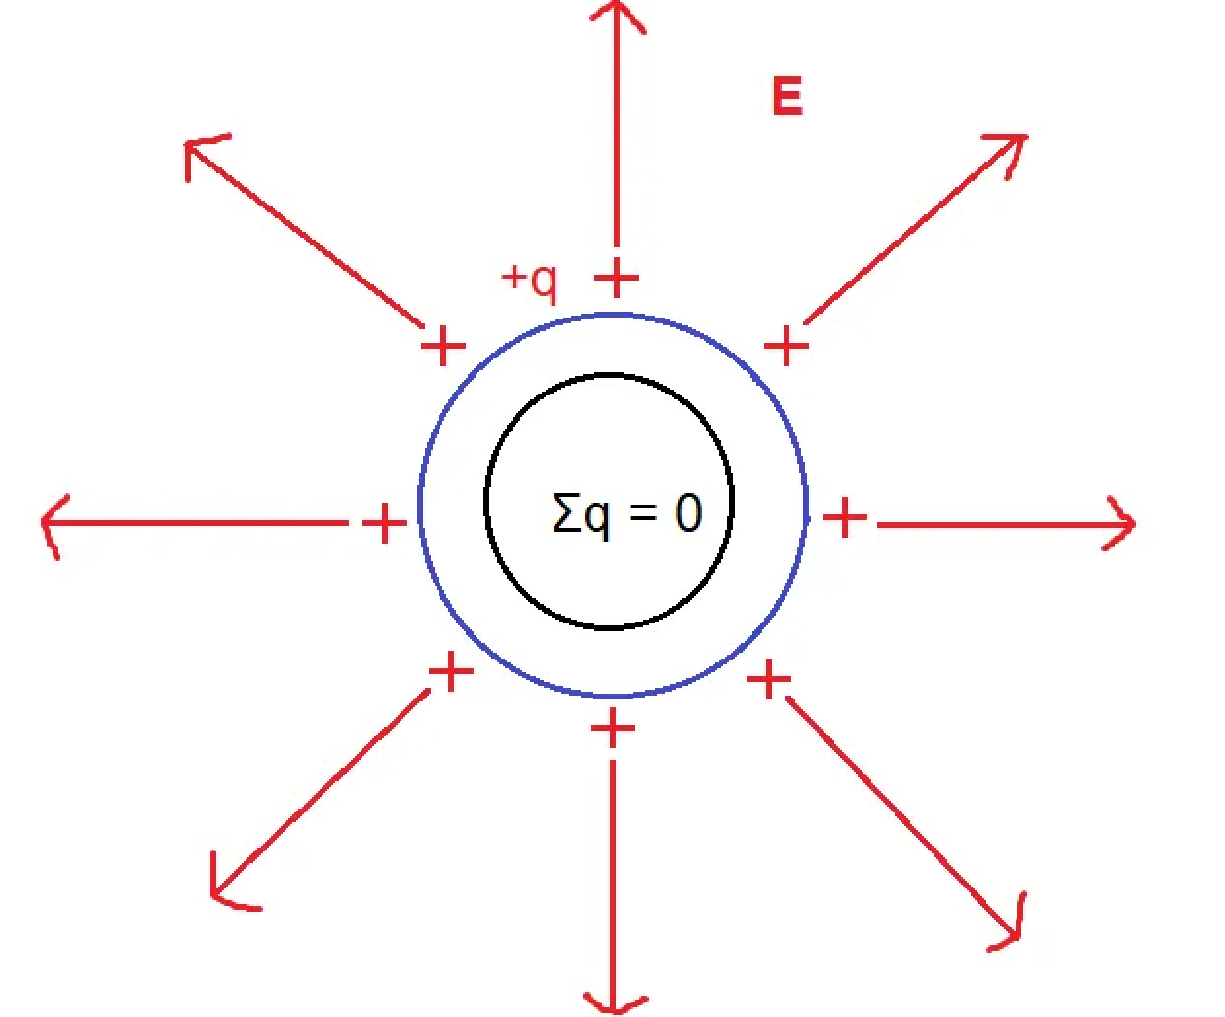
\includegraphics[height=250px]{photos/hollowtheory.png}
    \caption{Gaussian surface placed within hollow sphere (Tushar, 2020)}
    \label{fig:gaussiansurface}
\end{figure}
According to Gauss' law, any electric field experienced on the surface of this sphere would be proportional to the amount of charge enclosed within the Gaussian surface. In the case of this hypothetical sphere, there is no enclosed charge. 

$$\oint \vec{E} \cdot d\vec{A} = \frac{Q_{encl.}}{\epsilon_{0}}$$

$$\oint \vec{E} \cdot d\vec{A} = 0$$

for $\oint \vec{E} \cdot d\vec{A}$ to equal $0$, one of the two must be true:
1) the electric field is 0, and thus no charge exists on the inside surface of the hollow sphere, or
2) the dot product of the two vectors is $0$, meaning they are perpendicular.
Since both the hollow and Gaussian spheres are spherical, all $\vec{E}$ and $d\vec{A}$ vectors are parallel. This can only mean that the electric field is 0, and there would, in theory, be no charge on the inside surface of the hollow sphere.


\newpage
